\documentclass{beamer}
\usepackage[spanish]{babel}
\usetheme{metropolis}           % Use metropolis theme
\graphicspath{{images/}}

\usepackage{multicol}

\usepackage[default]{sourcesanspro}

\usepackage[scale=2]{ccicons}


\hypersetup{
    colorlinks=true,
    linkcolor=black,
    filecolor=magenta,
    urlcolor=cyan,
}

\title{MH: Práctica 4\\
			PAR - Estudio y propuesta de metaheurística propia}


\date{\today}
\author{Antonio David Villegas Yeguas}
\institute{Universidad de Granada\\
\medskip
\textit{advy99@correo.ugr.es}
}
\setbeamertemplate{caption}{\raggedright\insertcaption\par}

\begin{document}

 \maketitle

\begin{frame}{Índice}
\tableofcontents
\end{frame}
  
  
\section{Inspiración}
\begin{frame}{Inspiración: Filosofía de Nietzsche}

	\begin{minipage}{0.3\textwidth}
    	\begin{figure}
   		 	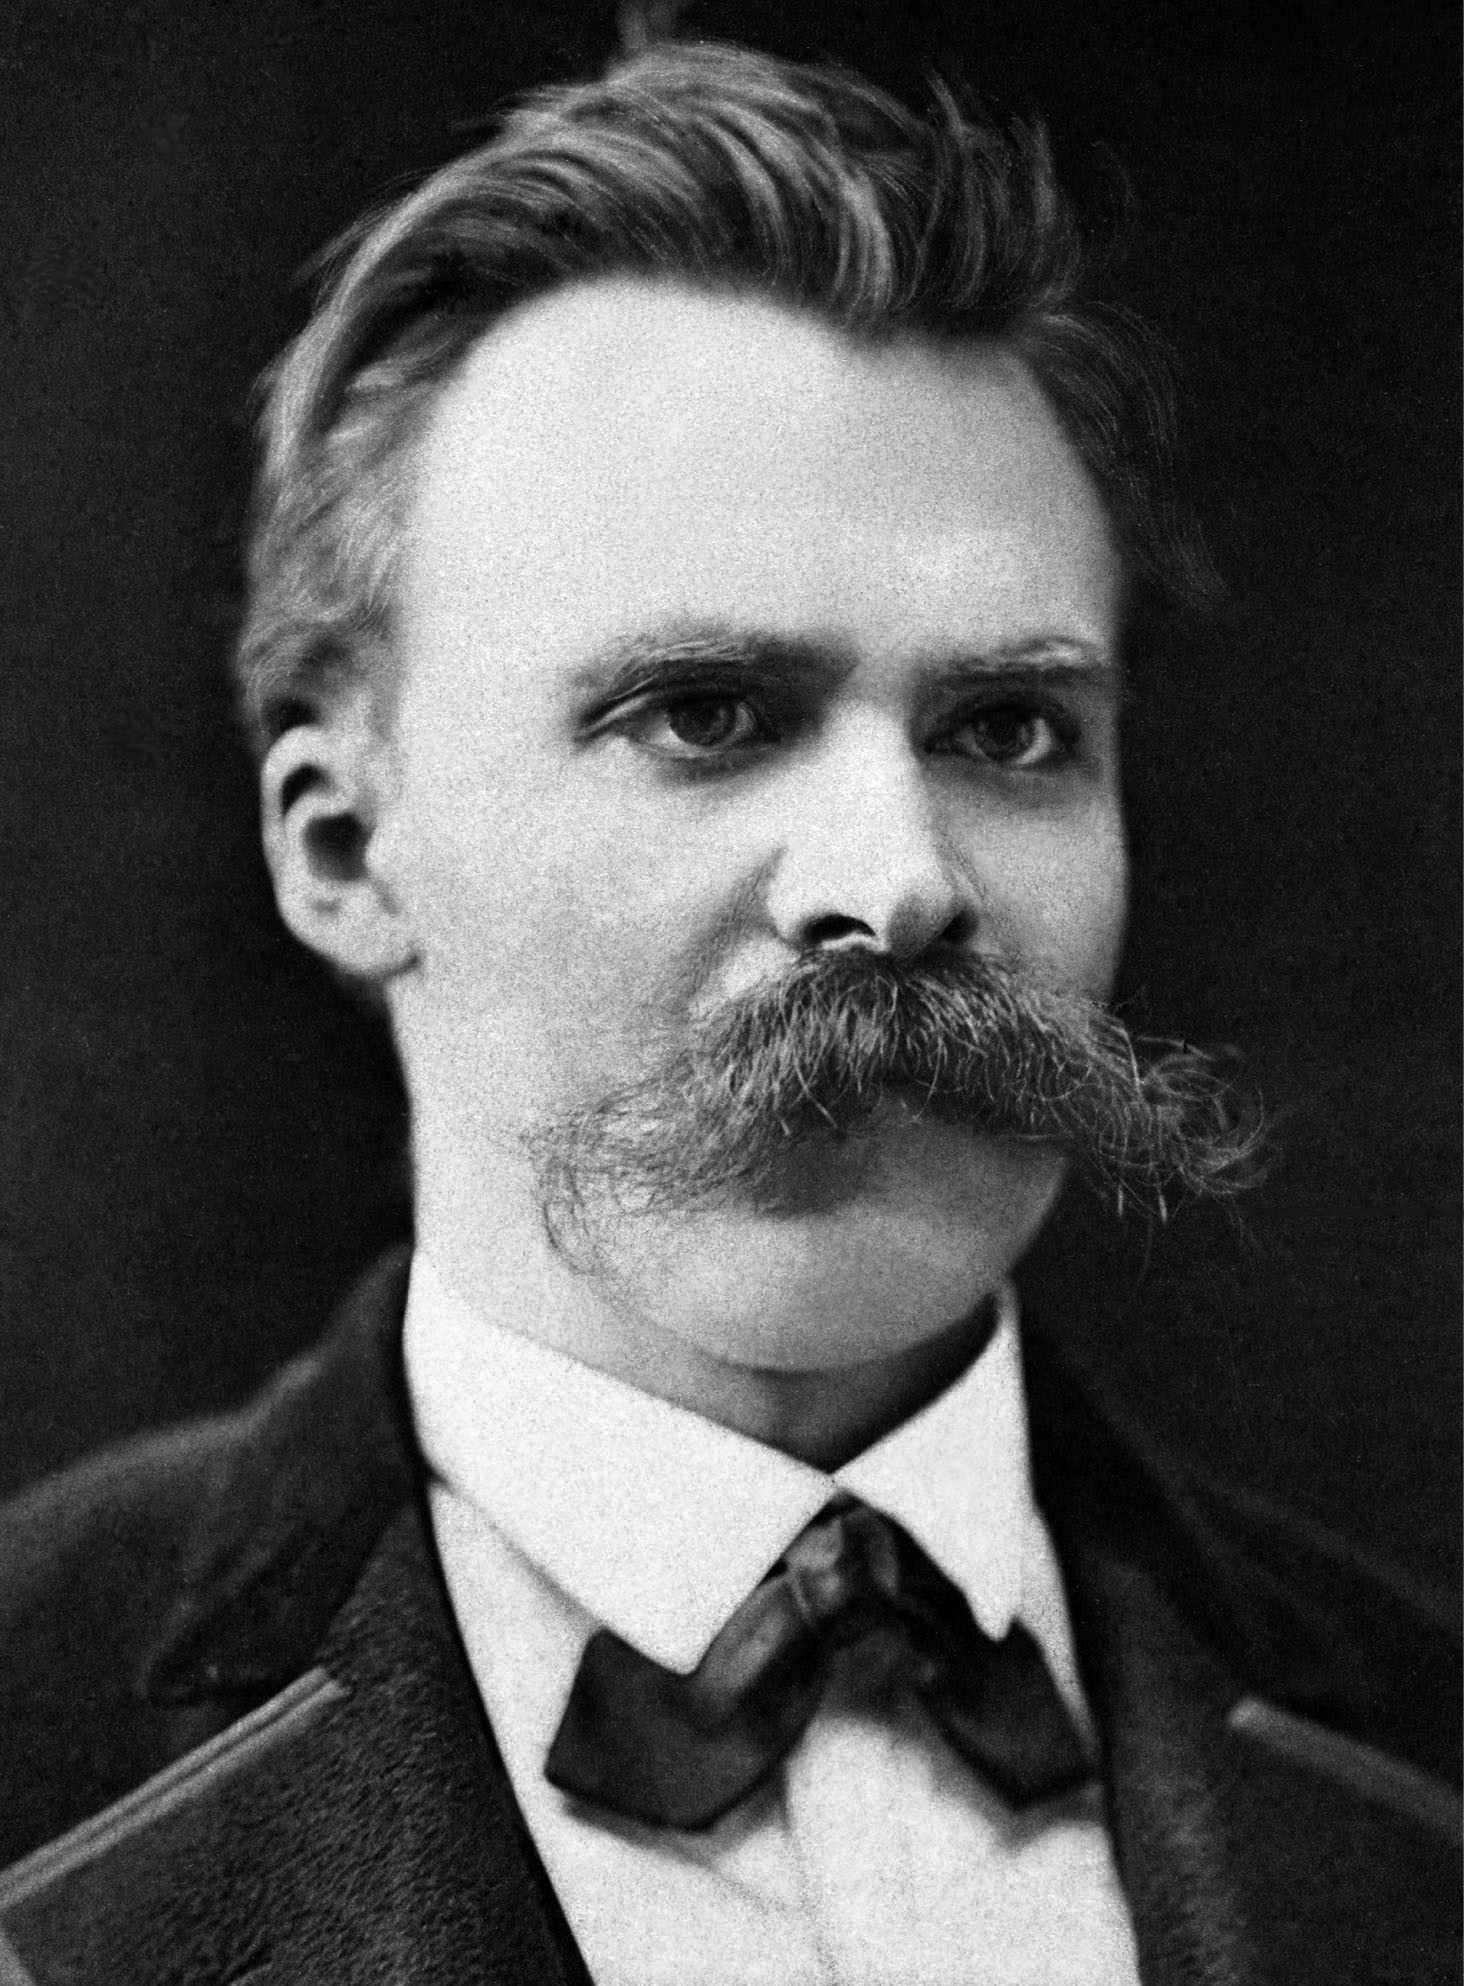
\includegraphics[scale=0.26]{nietzsche.jpg}
    		\caption{\footnotesize{Friedrich Nietzsche 15/10/1844 - 25/09/1900}}
   	
    	\end{figure}
    	
    \end{minipage}
    \hfill
	\begin{minipage}{0.6\textwidth}	
    	Idea obtenida de la filosofía de Nietzsche:
    
    	\begin{itemize}
			\item Sociedad sumida en nihilismo existencial. Desvalorización de los valores morales.
			\item Búsqueda del superhombre. Ser superior capaz de crear una moral propia, nuevos valores morales.
    	\end{itemize}
	\end{minipage}
	
\end{frame}
  
  
  
\section{Propuesta}
  
\begin{frame}{Propuesta:}
Siguiendo la idea de Nietzsche, algoritmo con dos poblaciones:

\begin{enumerate}
	\item Población sumida en el nihilismo: Exploración del entorno. Búsqueda de mejores zonas del espacio de búsqueda. Intentar salir del nihilismo.
	\item Población con superhombre: Explotación del entorno. La mejor solución hará de superhombre, el resto de soluciones intentarán parecerse a esta solución.
\end{enumerate}

\end{frame}  
  
  
  
\section{Implementación}
  
\section{Más información}
  
\begin{frame}{Más información: Código y documentación}

	Código disponible en: 
	
	\begin{center}
		\url{https://github.com/advy99/MH}	
	\end{center}
	
	Puedes descargar cada práctica con su respectiva documentación en:
	
	\begin{center}
		\url{https://github.com/advy99/MH/releases}	
	\end{center}

	
\end{frame}	  
  
\begin{frame}{Más información: Licencias}
  
	Toda la documentación se encuentra sobre la licencia
 	\href{https://creativecommons.org/licenses/by-nc-sa/4.0/deed.es}{Creative Commons
	Reconocimiento NoCommercial-CompartirIgual 4.0}.

	\begin{center}\ccbyncsa\end{center}

	\vspace{1cm}

	Mientras que el código se encuentra bajo la licencia \href{https://www.gnu.org/licenses/old-licenses/gpl-2.0.html}{GNU GPLv2}
  
\end{frame}


\end{document}